\documentclass[12pt]{article}
 
\usepackage[margin=1in]{geometry} 
\usepackage{amsmath,amsthm,amssymb,amsfonts}
\usepackage{color}
\usepackage{graphicx}
\graphicspath{ {Images/} }
\usepackage{float}
\setlength{\parskip}{1em}
\usepackage{cancel}
\usepackage{longtable}
\usepackage{algorithm}
\usepackage{algpseudocode}
\usepackage{pgf,tikz,pgfplots}
\pgfplotsset{compat=1.15}
\usepackage{mathrsfs}
\usetikzlibrary{arrows}
\pagestyle{empty}
\begin{document}

\section*{Problem 1}

This is a pedagogical toy problem. It is designed to show how Process and Pipe objects from the multiprocessing module on Python can be used in a separable optimisation problem.

The following is the separable unconstrained optimisation problem to be solved:
\begin{align*}
\min_{x_1,x_2,x_3}\qquad& x_1^2+x_2^2+2x_3^2,
\end{align*}
where $x_1,x_2,x_3\in\mathbb{R}$. Let $x_1$ and $x_2$ both be private variables, i.e., they can only be accessed by Agent 1 and Agent 2 respectively. Let $x_3$ be a shared or public variable that can be accessed by all agents. The minimiser of this problem is obviously $(x_1^*,x_2^*,x_3^*)=(0,0,0)$, but remember, the point of this problem is really to give Python's multiprocessing module a test run on an optimisation problem. 

By applying a change of variables, the cost function can be separated and the new formulation of the problem will be
\begin{align*}
\min_{x_1,\xi_1,x_2,\xi_2}\qquad& [x_1^2+\xi_1^2]+[x_2^2+\xi_2^2]\\
s.t.\qquad&\xi_1=\xi_2,
\end{align*}
where $x_1,\xi_1,x_2,\xi_2\in\mathbb{R}$. The dual function will then be
\begin{align*}
q(\lambda)&=q_1(\lambda)+q_2(\lambda)\\
&=\inf_{x_1,\xi_1}[x_1^2+\xi_1^2-\lambda\xi_1]+\inf_{x_2,\xi_2}[x_2^2+\xi_2^2+\lambda\xi_2].
\end{align*}
The minimisers of $[x_1^2+\xi_1^2-\lambda\xi_1]$ and $[x_2^2+\xi_2^2+\lambda\xi_2]$ will be $(x_1^*,\xi_1^*)=(0,\lambda/2)$ and $(x_2^*,\xi_2^*)=(0,-\lambda/2)$ respectively. The algorithm will be as follows:

\begin{itemize}
	\item At step $k=0$, some master processor chooses an initial $\lambda(0)=1.0$ and sends $\lambda(0)$ to Agents 1 and 2. Agent 1 calculates $\xi_1^*(0)=\lambda(0)/2$, while (in parallel) Agent 2 calculates $\xi_2^*(0)=-\lambda(0)/2$. Agents 1 and 2 send $\xi_1^*(0)$ and $\xi_2^*(0)$ back to the master processor.
	\item At step $k=1$, the master processor updates $\lambda(1)=\lambda(0)-\alpha(\xi_1^*(0)-\xi_2^*(0))$ and sends $\lambda(1)$ to Agents 1 and 2. Agent 1 calculates $\xi_1^*(1)=\lambda(1)/2$, while (in parallel) Agent 2 calculates $\xi_2^*(1)=-\lambda(1)/2$. Agents 1 and 2 send $\xi_1^*(1)$ and $\xi_2^*(1)$ back to the master processor.
	\item Keep looping until $\xi_1^*(k)-\xi_2^*(k)$ is small enough, or we reach some chosen maximum number of iterations.
\end{itemize}


\subsection*{Computational Overhead}

There is some computational overhead to spawn a Process on Python. The parallel processes in this problem are computationally cheap compared to this overhead; Agent 1 just needs to compute $\xi_1^*(k)=\lambda(k)/2$ while Agent 2 only needs to compute $\xi_2^*(k)=-\lambda(k)/2$ each iteration. Thus, it is faster to just carry out the processes in series.

As a sanity check, let's simulate a more ``difficult'' problem, where the minimisers $\xi_1^*(k)$ and $\xi_2^*(k)$ may be more computationally expensive to compute. This can be done by introducing a for-loop that in the parallel processes so that on top of calculating $\xi_1^*(k)$ and $\xi_2^*(k)$, the agents must also loop through a large ``dummy'' calculation. When the ``dummy'' for-loop is made large enough (of the order $1000000$ iterations), we start to see the serial method overtake the parallel method in terms of completion time.

\begin{figure}[H]
	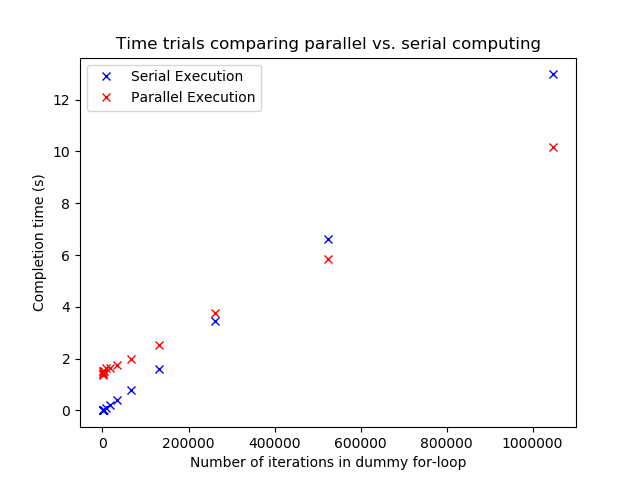
\includegraphics[scale=1]{Problem1-TimeTrial.png}
\end{figure}

Thus, we passed the sanity check. For parallel computing to finish faster than serial computing, the cost of computation per process must be larger the computational cost of spawning that process. In terms of our optimisation problem, the decomposed dual function must be decomposed into smaller functions whose minimisers are found through sufficiently complex computations, in order to observe any fruitful results from using parallel computing.

\subsection*{Convergence of Algorithm}

We get convergence to $(x_1^*,x_2^*,x_3^*)=(0,0,0)$ as expected. It turns out that convergence occurs regardless of how the variable $x_3^2$ in the cost function is separated. Given $f=x_1^2+x_2^2+2x_3^2$, convergence occurs for $f=[x_1^2+2ax_3^2]+[x_2^2+2(1-a)x_3^2]$ for all $a\in(0,1)$. This will be observed in more detail, in Problem 2.

\begin{figure}[H]
	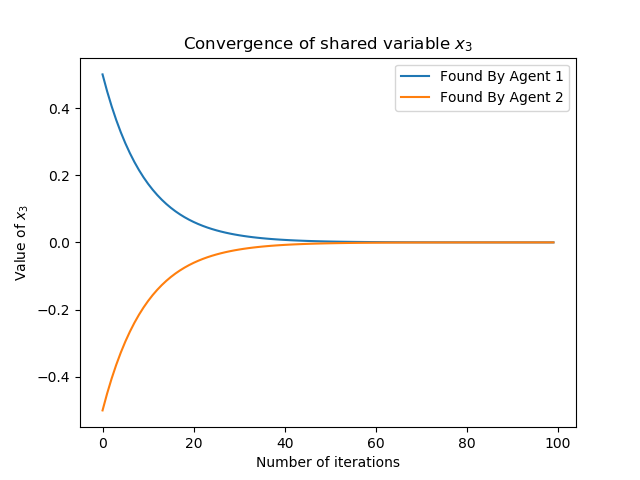
\includegraphics[scale=1]{Problem1-Convergence.png}
\end{figure}

\subsection*{How to Run}

\subsubsection*{The above examples}

Make sure you are in the correct directory. Then to run the test that generated the above plots, execute the \textbf{main.py} file, i.e. use the command

\noindent \textbf{$>>>$python main.py}

\subsubsection*{Function Descriptions}

The function \textbf{parallel.do\_parallel}, description.

Syntax: do\_parallel(max\_iter,alpha,size\_problem=0,verbose=False)

Parameter values:
\begin{itemize}
	\item max\_iter, Required. Number of iterations for the subgradient method.
	\item alpha, Required. Step size for the subgradient method.
	\item size\_problem, Default 0. Number of iterations for the dummy for-loop.
	\item verbose, Default False. Print results to screen.
\end{itemize}

Outputs:
\begin{itemize}
	\item Output 1. List containing $\xi_1^*$ for all iterations of the subgradient method.
	\item Output 2. List containing $\xi_2^*$ for all iterations of the subgradient method.
	\item Output 3. Completion time.
\end{itemize}




\end{document}